\section{Appendices}

This section details validation of the use of simplified likelihoods in two example searches for BSM physics at CMS. 
\emph{The section is not intended for public dissemination and should be considered as internal material only.}

\subsection{Monojet/V search -- EXO-16-037}

The simplified likelihood approach has been validated in a search dark matter (DM) in  
13\TeV proton-proton collision events with a large missing transverse momentum and jets resulting from radiation 
of a gluon or a vector boson~\cite{CMS-PAS-EXO-16-037}.

The search comprises two categories of events that are defined by the nature of the jets in the event. 
The first category, labelled mono-V, selects events which contain a ``fat-jet'' with a mass and substructure 
consistent with that of a hadrinically decaying W or Z boson. The second category, the monojet category, 
includes events failing the selection of the first but containing at least one high transverse momentum jet. 
In both categories, the magnitude of the missing transverse momentum, $\ETmiss$, is used to further discriminate the signal from the background.  
Each category is divided into several search regions defined as intervals in $\ETmiss$, 7 in the mono-V category and 22 in the 
monojet category making a total of 29 search regions.  The results of the search are interpreted 
in terms of simplified models for DM production~\cite{simplified1,Buchmueller:2013dya,Buchmueller:2014yoa},
mediated via vector, axial vector, scalar or pseudoscalar interactions and 
in terms of a Higgs boson decaying to invisible particles. 

Figure~\ref{fig:monojetv} shows the number of events in each of the $\ETmiss$ intervals observed in each of two event 
categories as well as the total number of expected background events and the relative contribution of each source of background. The same information 
is tabulated in Tables~\ref{tab:monojettab} and~\ref{tab:monovtab}. 

\begin{figure}[hbt!]
  \begin{center} 
   \subfloat[][]{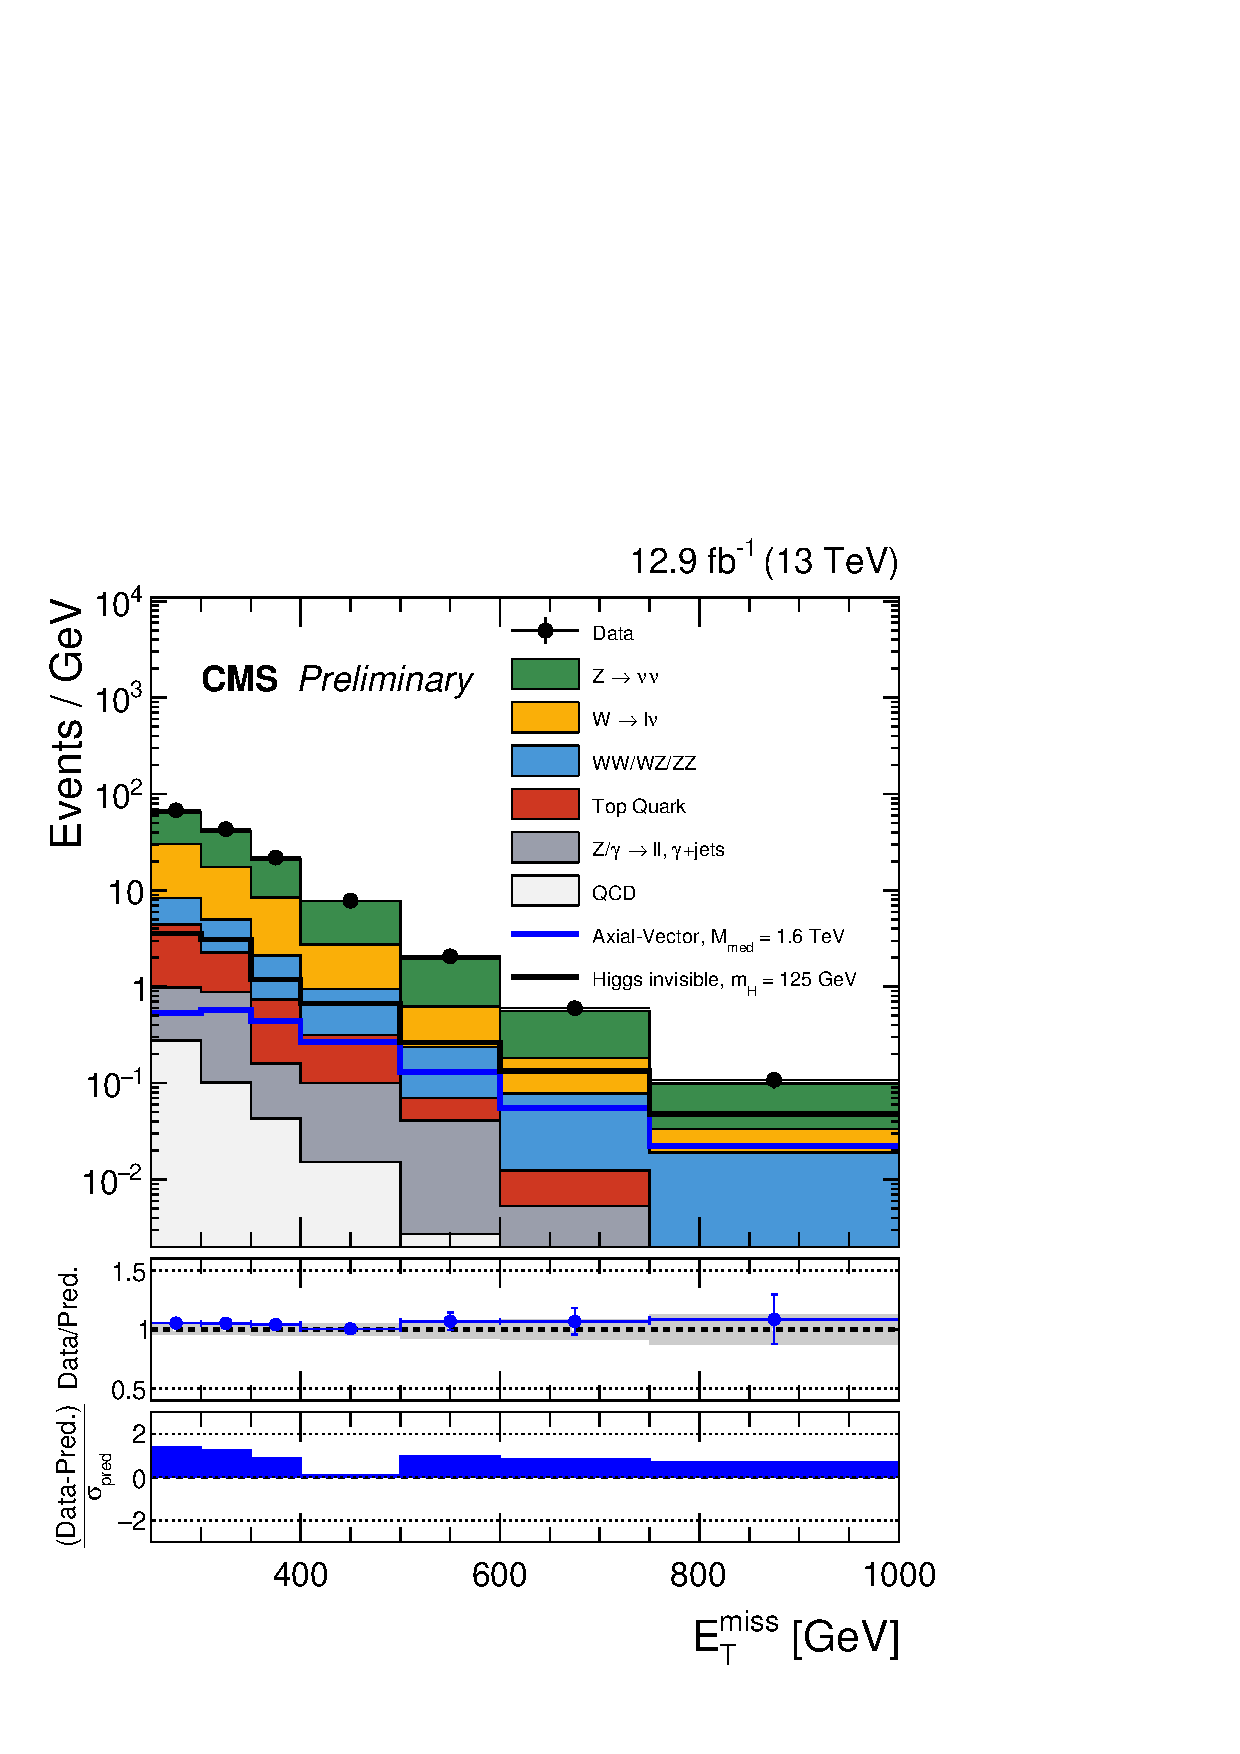
\includegraphics[width=1.2\cmsFigWidth]{figures/postfit_sig_MV_SRmask.pdf}}
   \subfloat[][]{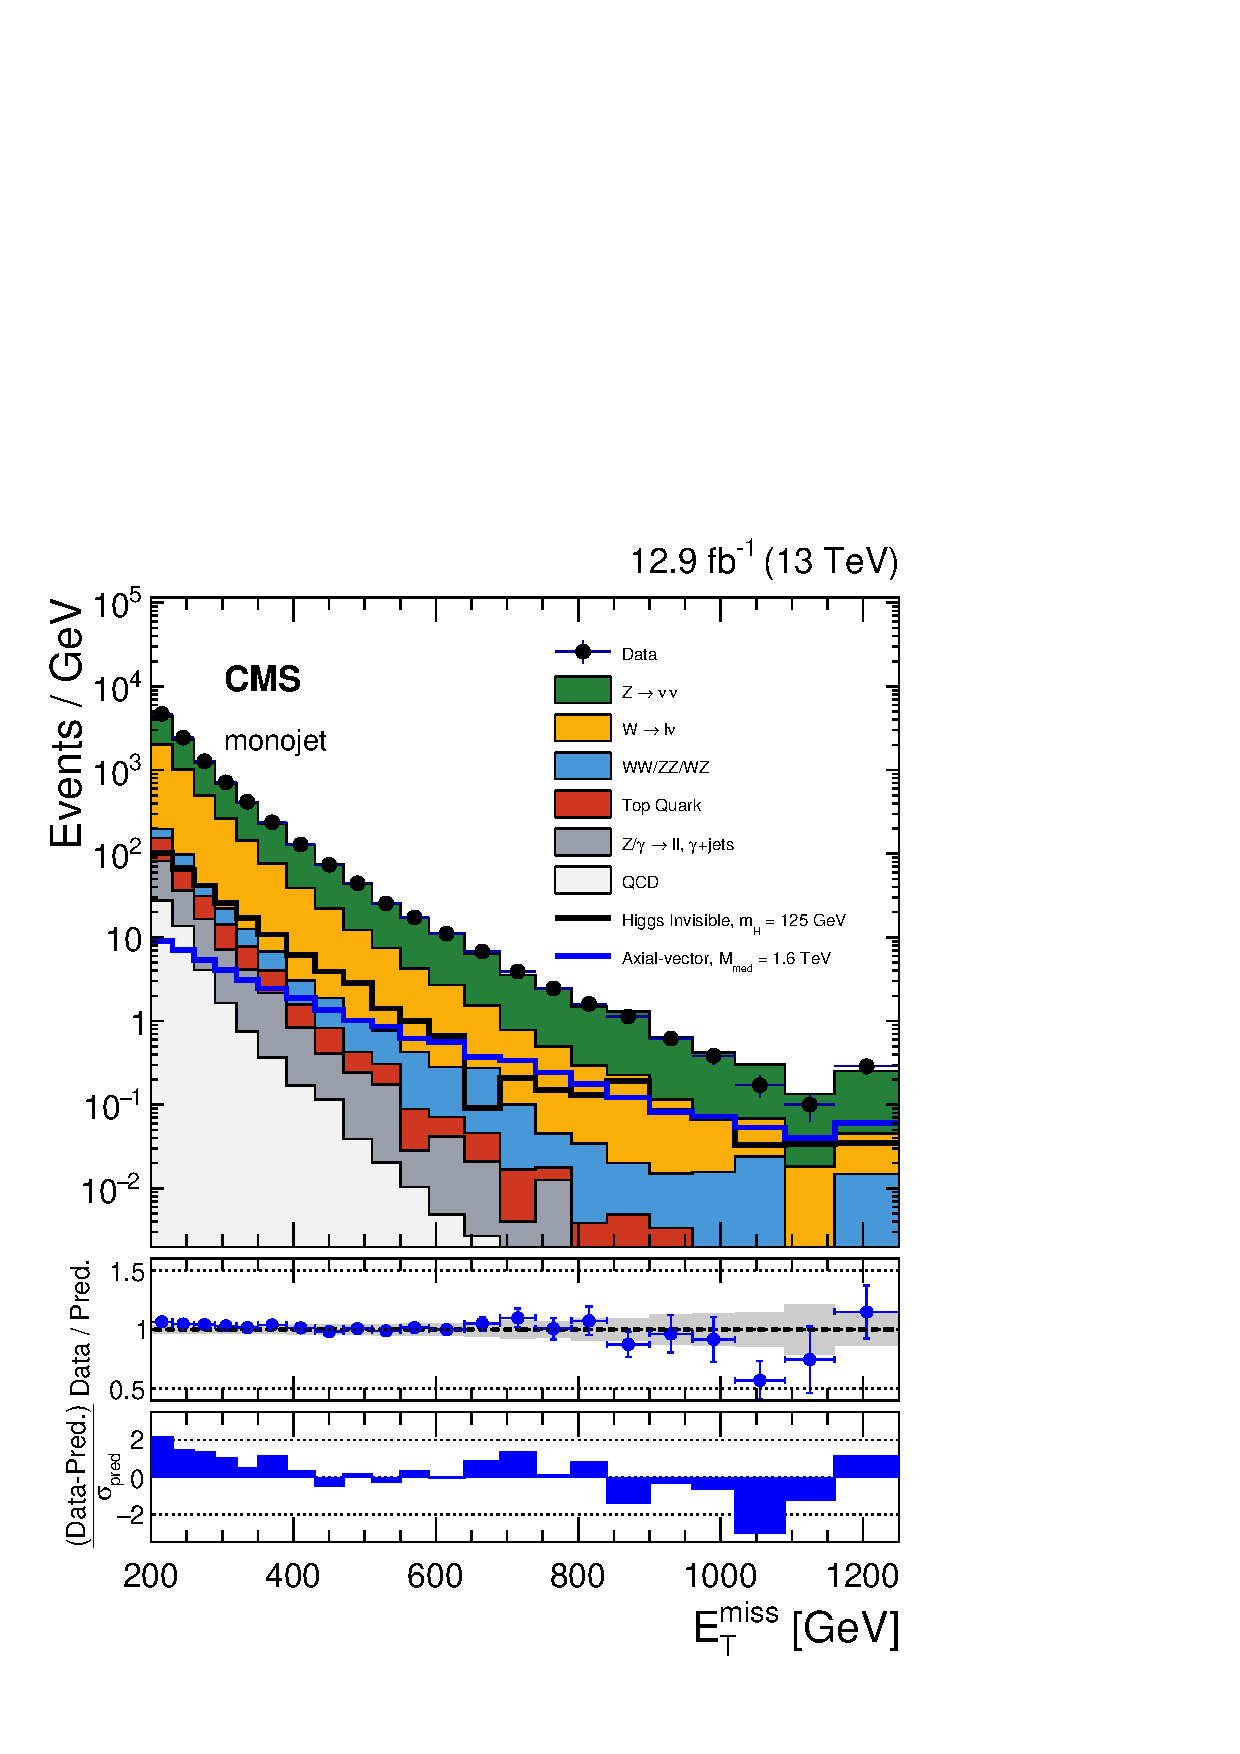
\includegraphics[width=1.2\cmsFigWidth]{figures/monojet_PULLS_MASKED_prefit_postfit_signal.pdf}}
\caption{
      Observed number of events in each \ETmiss interval in the (a) mono-V and (b) monojet categories compared with the background expectations for various SM processes.
      The last bin includes all events with \ETmiss$ > 1160 \GeV$ for the monojet category and \ETm$ > 750 \GeV$ for the mono-V category.
      The expected background distributions are evaluated after performing a combined fit to the data in all the control regions, but not including the search regions.
      Expected signal distributions from the 125 GeV Higgs boson decaying exclusively to invisible particles, and a 1.6 TeV axial-vector mediator decaying to 1 GeV DM particles, are overlaid.
      The ratio of data with the background prediction is shown for both the monojet and mono-V signal regions.
      The gray bands in these ratio plots indicate the uncertainty in the background prediction and are dervied as the square root of the variance of the expected number of background events.
      Finally the difference between data and the background prediction relative to the uncertainty in the prediction,
      are also shown in the lower panels.
   }
   \label{fig:monojetv} 
  \end{center}
\end{figure}


\begin{table}[!htb]
\caption{Observed and expected event yields in each \ETmiss 
search region for various background processes 
in the mono-V category. The background yields and the 
corresponding uncertainties are obtained after performing a combined fit to data in all the 
control regions and do not use data in any of the search regions.
	 }
 \begin{center}
 \scriptsize
 \begin{tabular}{c|c|c|c|c|c|c|c}
 \hline
 \ETMiss (GeV) & Data & $\mathrm{Z} \rightarrow \nu\nu$ & $\mathrm{W} \rightarrow \ell\nu$ & Top quark & Dibosons & Other & Total Bkg. \\
 \hline
250--300 & 3395 & 1700 $\pm$ 88  & 1100  $\pm$ 65  & 171 $\pm$ 24   & 195 $\pm$ 35    & 49.4 $\pm$ 10.8 & 3220 $\pm$ 130 \\
300--350 & 2162 & 1180 $\pm$ 68  & 627   $\pm$ 37  & 68.8 $\pm$ 9.7 & 135 $\pm$ 24    & 44.2 $\pm$ 7.2  & 2050 $\pm$ 88 \\
350--400 & 1093 & 629 $\pm$ 37   & 314   $\pm$ 21  & 28.9 $\pm$ 4.1 & 68.5 $\pm$ 12   & 8.0 $\pm$ 1.8   & 1048 $\pm$ 51 \\
400--500 & 780  & 500 $\pm$ 33   & 181   $\pm$ 13  & 21.4 $\pm$ 3.0 & 62.8 $\pm$ 11   & 10.1 $\pm$ 1.8  & 775  $\pm$ 40 \\
500--600 & 207  & 131 $\pm$ 12   & 38.5  $\pm$ 3.4 & 2.9 $\pm$ 0.4  & 16.8 $\pm$ 3.0  & 4.1 $\pm$ 0.8   & 193  $\pm$ 14 \\
600--750 & 90   & 57.1 $\pm$ 5.9 & 15.6 $\pm$ 1.6  & 1.0 $\pm$ 0.1  & 9.8 $\pm$ 1.7   & 0.8 $\pm$ 0.1   & 84.2 $\pm$ 6.9 \\
750--1000 & 27  & 16.5 $\pm$ 2.7 & 3.6  $\pm$ 0.6  & -              & 4.7 $\pm$ 0.8   & 0.01 $\pm$ 0.01 & 24.8 $\pm$ 3.1 \\
 \hline
\end{tabular}
\end{center}
\label{tab:monovtab}
\end{table}



\begin{table}[htb]
\caption{Observed and expected event yields in each \ETmiss search region for various background processes in the monojet category. The background yields and the
         corresponding uncertainties are obtained after performing a combined fit to data in all the control regions and do not use data in any of the search regions.
	 }
 \begin{center}
 \scriptsize
 \begin{tabular}{c|c|c|c|c|c|c|c}
 \hline
 \ETmiss (GeV) & Data & $\mathrm{Z} \rightarrow \nu\nu$ & $\mathrm{W} \rightarrow \ell\nu$ & Top quark & Dibosons & Other & Total Bkg. \\
 \hline
200--230 & 140642 & 71300 $\pm$ 2200 & 54600 $\pm$ 2300 & 2140 $\pm$ 320  & 1320 $\pm$ 220   & 2470 $\pm$ 310   & 132100 $\pm$ 4000 \\
230--260 & 73114  & 39500 $\pm$ 1300 & 27500 $\pm$ 1200 & 1060 $\pm$ 160  & 790 $\pm$ 130    & 1090 $\pm$ 130   & 69900  $\pm$ 2200 \\
260--290 & 38321  & 21900 $\pm$ 670  & 13600 $\pm$ 550  & 440 $\pm$ 65    & 364 $\pm$ 61     & 498 $\pm$  65    & 36800  $\pm$ 1100 \\
290--320 & 21417  & 12900 $\pm$ 400  & 7300 $\pm$ 290   & 210 $\pm$ 31    & 235 $\pm$ 40     & 216 $\pm$ 30     & 20780  $\pm$ 630 \\
320--350 & 12525  & 8000 $\pm$ 280   & 4000 $\pm$ 170   & 107 $\pm$ 16    & 145 $\pm$ 24     & 124 $\pm$ 18     & 12340 $\pm$ 400 \\
350--390 & 9515   & 6100 $\pm$ 220   & 2800 $\pm$ 130   & 74  $\pm$ 11    & 111 $\pm$ 19     & 87  $\pm$ 13     & 9160 $\pm$ 320 \\
390--430 & 5174   & 3500 $\pm$ 160   & 1434 $\pm$ 66    & 30.1 $\pm$ 4.5  & 58.4 $\pm$ 9.9   & 33.4 $\pm$ 5.3   & 5100 $\pm$ 200 \\
430--470 & 2947   & 2100 $\pm$ 98    & 816 $\pm$ 37     & 16.6 $\pm$ 2.5  & 42.4 $\pm$ 7.1   & 16.3 $\pm$ 2.7   & 3000 $\pm$ 120 \\
470--510 & 1777   & 1300 $\pm$ 66    & 450 $\pm$ 20     & 7.4 $\pm$ 1.1   & 24.6 $\pm$ 4.1   & 9.6 $\pm$ 1.6    & 1763 $\pm$ 79 \\
510--550 & 1021   & 735 $\pm$ 39     & 266 $\pm$ 13     & 5.2 $\pm$ 0.8   & 18.5 $\pm$ 3.1   & 7.0 $\pm$ 1.3    & 1032 $\pm$ 48 \\
550--590 & 694    & 513 $\pm$ 31     & 152 $\pm$ 8      & 2.4 $\pm$ 0.4   & 13.5 $\pm$ 2.3   & 1.1 $\pm$ 0.3    & 683 $\pm$ 37 \\
590--640 & 554    & 419 $\pm$ 23     & 120 $\pm$ 6      & 1.5 $\pm$ 0.2   & 10.6 $\pm$ 1.8   & 2.1 $\pm$ 0.4    & 554 $\pm$ 28 \\
640--690 & 339    & 246 $\pm$ 16     & 62.8 $\pm$ 3.8   & 1.3 $\pm$ 0.2   & 11.4 $\pm$ 1.9   & 1.0 $\pm$ 0.2    & 322 $\pm$ 19 \\
690--740 & 196    & 139 $\pm$ 11     & 34.2 $\pm$ 2.4   & 0.6 $\pm$ 0.1   & 4.2 $\pm$ 0.7    & 0.20 $\pm$ 0.07  & 178 $\pm$ 13 \\
740--790 & 123    & 97.2 $\pm$ 7.2   & 22.7 $\pm$ 1.7   & 0.22 $\pm$ 0.03 & 1.4 $\pm$ 0.2    & 0.63 $\pm$ 0.12  & 122 $\pm$ 8 \\
790--840 & 80     & 59.8 $\pm$ 5.8   & 12.9 $\pm$ 1.2   & 0.13 $\pm$ 0.02 & 1.5 $\pm$ 0.3    & 0.05 $\pm$ 0.02  & 74.5 $\pm$ 6.6 \\
840--900 & 68     & 64.3 $\pm$ 6.4   & 12.3 $\pm$ 1.1   & 0.24 $\pm$ 0.04 & 0.92 $\pm$ 0.11  & 0.03 $\pm$ 0.01  & 77.8 $\pm$ 7.2 \\
900--960 & 37     & 31.5 $\pm$ 4.3   & 6.0 $\pm$ 0.7    & 0.21 $\pm$ 0.03 & 0.74 $\pm$ 0.10  & 0.01 $\pm$ 0.01  & 38.4 $\pm$ 4.8 \\
960--1020 & 23    & 20.8 $\pm$ 3.0   & 3.4 $\pm$ 0.5    & -               & 0.94 $\pm$ 0.23  & 0.01 $\pm$ 0.01  & 25.1 $\pm$ 3.4 \\
1020--1090 & 12   & 16.3 $\pm$ 2.6   & 3.1 $\pm$ 0.5    & 0.04 $\pm$ 0.01 & 1.6  $\pm$ 0.3   & 0.01 $\pm$ 0.01  & 21.1 $\pm$ 3.0 \\
1090--1160 & 7    & 8.1 $\pm$ 1.8    & 1.3 $\pm$ 0.3    & -               & -                & -                & 9.4 $\pm$ 1.9 \\
1160--1250 & 26   & 18.6 $\pm$ 2.7   & 2.7 $\pm$ 0.4    & -               & 1.3 $\pm$ 0.2    & -                & 22.6 $\pm$ 3.0 \\
 \hline
\end{tabular}
\end{center}
\label{tab:monojettab}
\end{table}


The dominant backgrounds in this search are derived by defining several control regions in the data and simultaneously fitting for their contribution 
in the control and search regions. The full procedure is described in detail in Secion 4 of Ref.~\cite{CMS-PAS-EXO-16-037}. The smaller backgrounds are estimated from 
simulation, tuned using data. The full likelihood model used in this search contains $\mathcal{O}(100)$ nuisance parameters relating to theoretical 
extrapolations between the control regions and the search regions as well as experimental sytematic uncertainties on 
the lepton identification and jet reconstruction used. The full likelihood is therefore prohibitavely complicated, making its publication unfeasible. 
Instead, the simplified likelihood approach can be used. Figure~\ref{fig:fullcovariance} shows the correlation coefficeints, $\left\{\rho_{ij}\right\}_{i,j=1}^{29}$, between the total background 
rate in each of the 29 search regions. Both the correlations and the total expected background contributions are dervied without using the data in the 
search regions, allowing for construction of the simplified likelihood. Note that covariance matrix can be derived from the correlation coefficients and 
the variance (the square of the last colum in Tables~\ref{tab:monojettab} and~\ref{tab:monovtab}) since, 

\begin{align}
V_{ij} = \rho_{ij}\cdot\sigma_{i}\sigma_{j}, &&  \sigma_{k}^{2}=V_{kk}
\end{align}


\begin{figure}[hbt!]
  \begin{center} 
   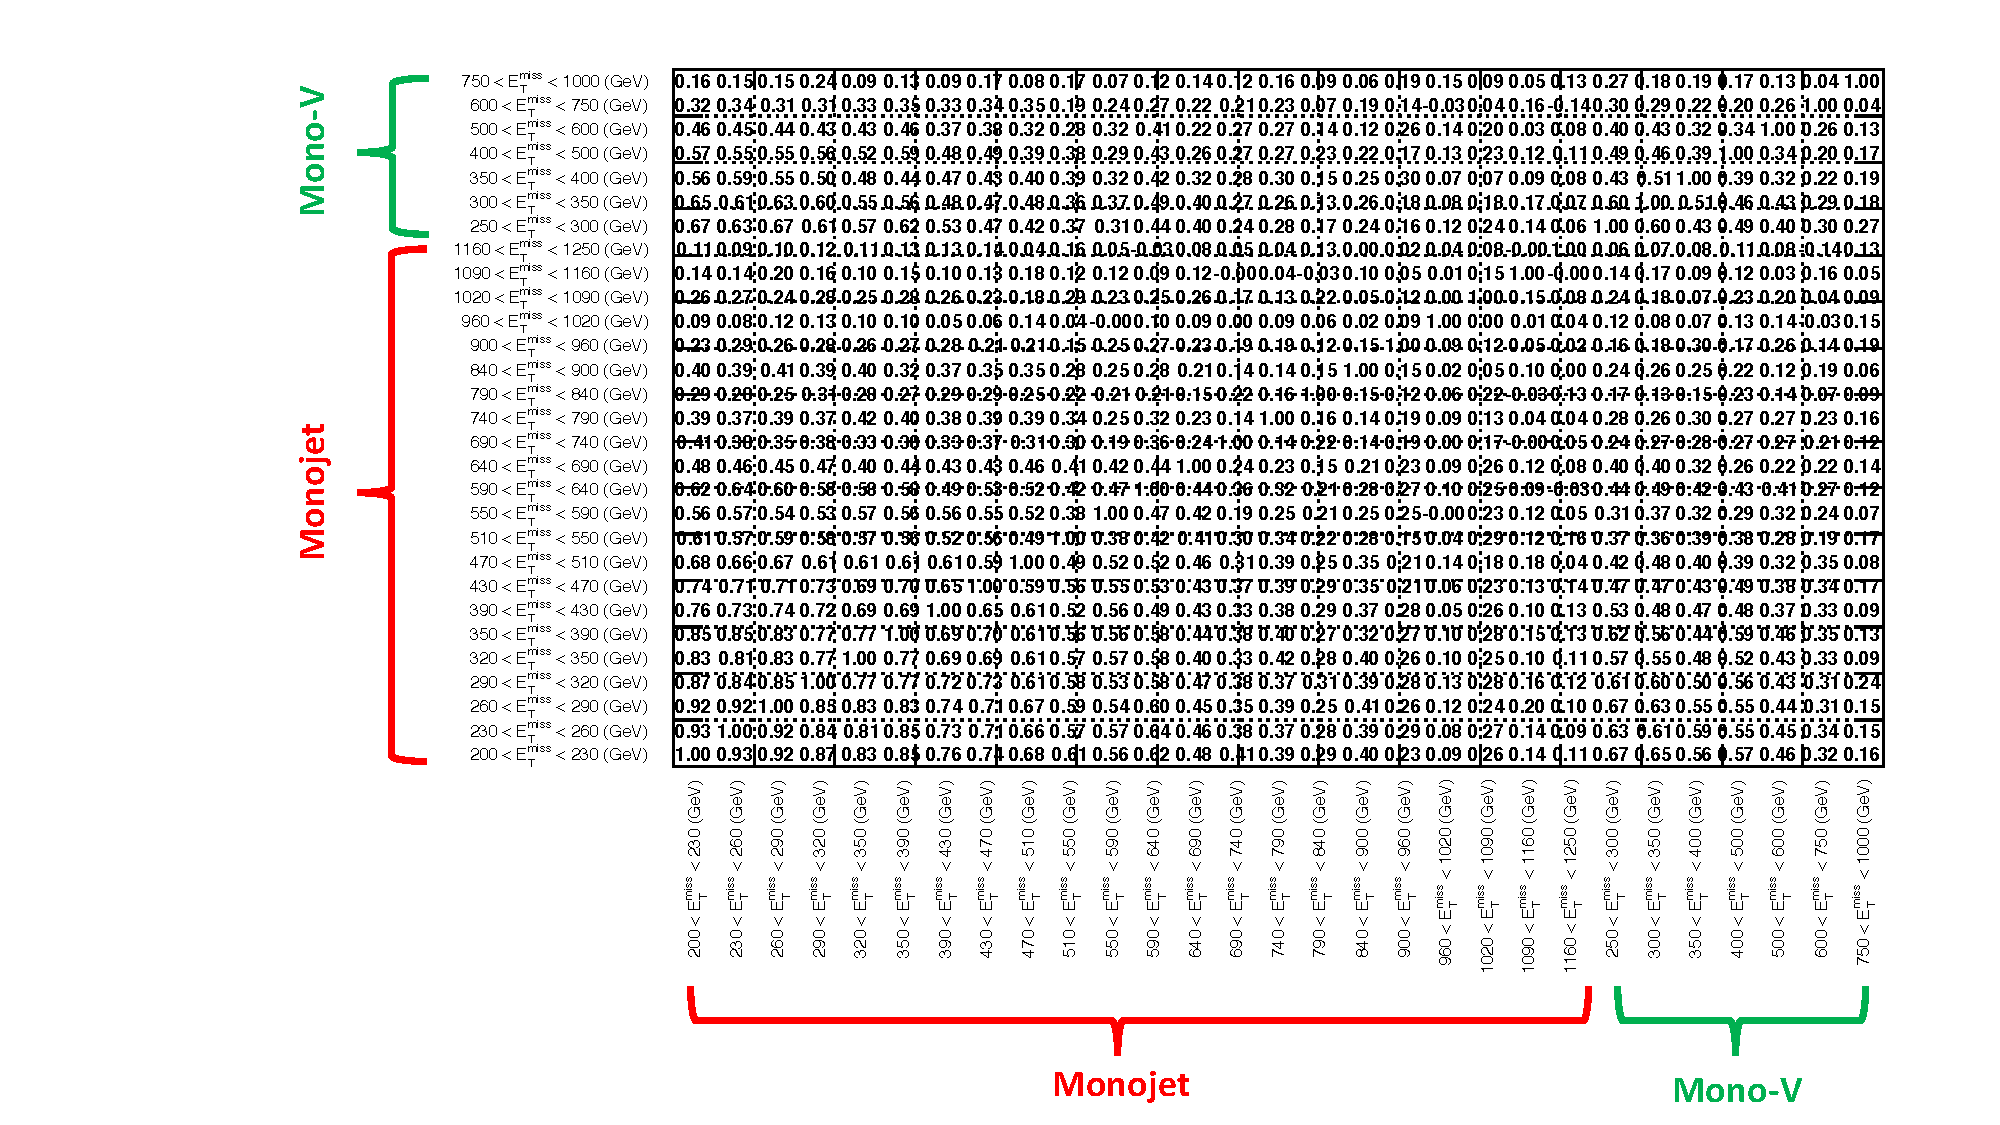
\includegraphics[width=2.6\cmsFigWidth]{figures/big_corr.pdf}
\caption{Correlation coefficients between the expected total background rates in the 29 search regions of the monojet and mono-V categories}
   \label{fig:fullcovariance} 
  \end{center}
\end{figure}


Figure~\ref{fig:lhscan-mj} shows a comparison of $q(\mu)$ as a function of $\mu$ for an example signal point in the simplified model parameter space. 
The results are compare to the ones obtained using 
the full likelihood and using the simplified likelihood, ignoring correlations between the background expectations. The results using an Asimov dataset assuming a signal 
strength of $\mu=1$ are also shown as these are used to calculate limits using the asymptotic approximations detailed in Ref.~\cite{Cowan:2010js}. 


\begin{figure}[hbt!]
  \begin{center} 
   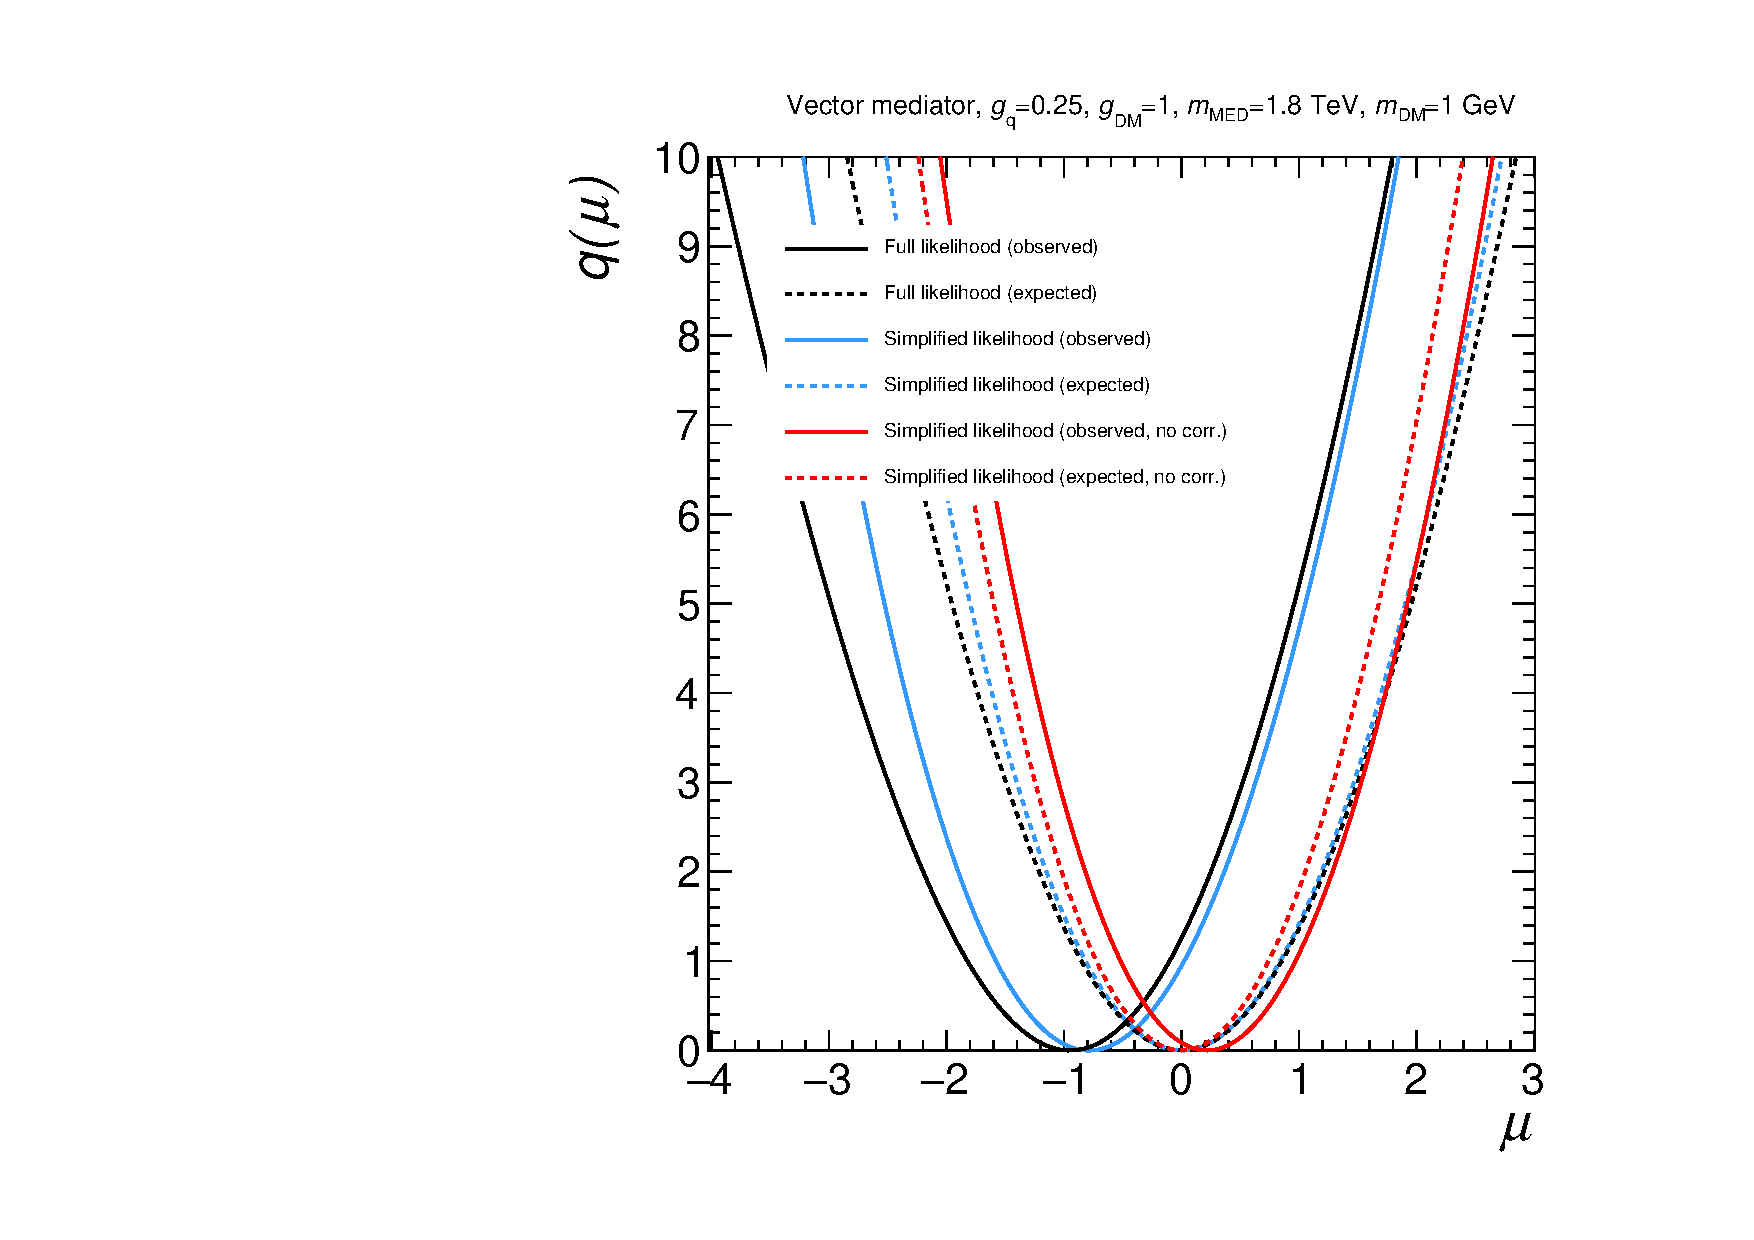
\includegraphics[width=1.5\cmsFigWidth]{figures/compare_mj_likelihoods.pdf}
   \caption{Scan of $q_{\mu}$ as a function of $\mu$ using the full and simplified likelioods and simplified likelihood ignoring background correlations. 
   The results are shown for the observed data and using an Asimov dataset assuming $\mu=1$.}
   \label{fig:lhscan-mj} 
  \end{center}
\end{figure}


Figure~\ref{fig:mulims} show a comparison of the 95\% confidence level upper limit on the signal strength, $\mu_{\mathrm{up}}^{95\%}$, as a function of 
the mass of a scalar or pseudoscalar mediator, $m_{\mathrm{MED}}$, for a fixed value of the coupling parameters and a fixed darm matter mass, $m_{\mathrm{DM}}=10$\GeV. 
The results are compared using the full likelihood and the simplified likelihood in the definition of the test statistic for both expected and observed upper limits. 


\begin{figure}[hbt!]
  \begin{center} 
  \subfloat[][]{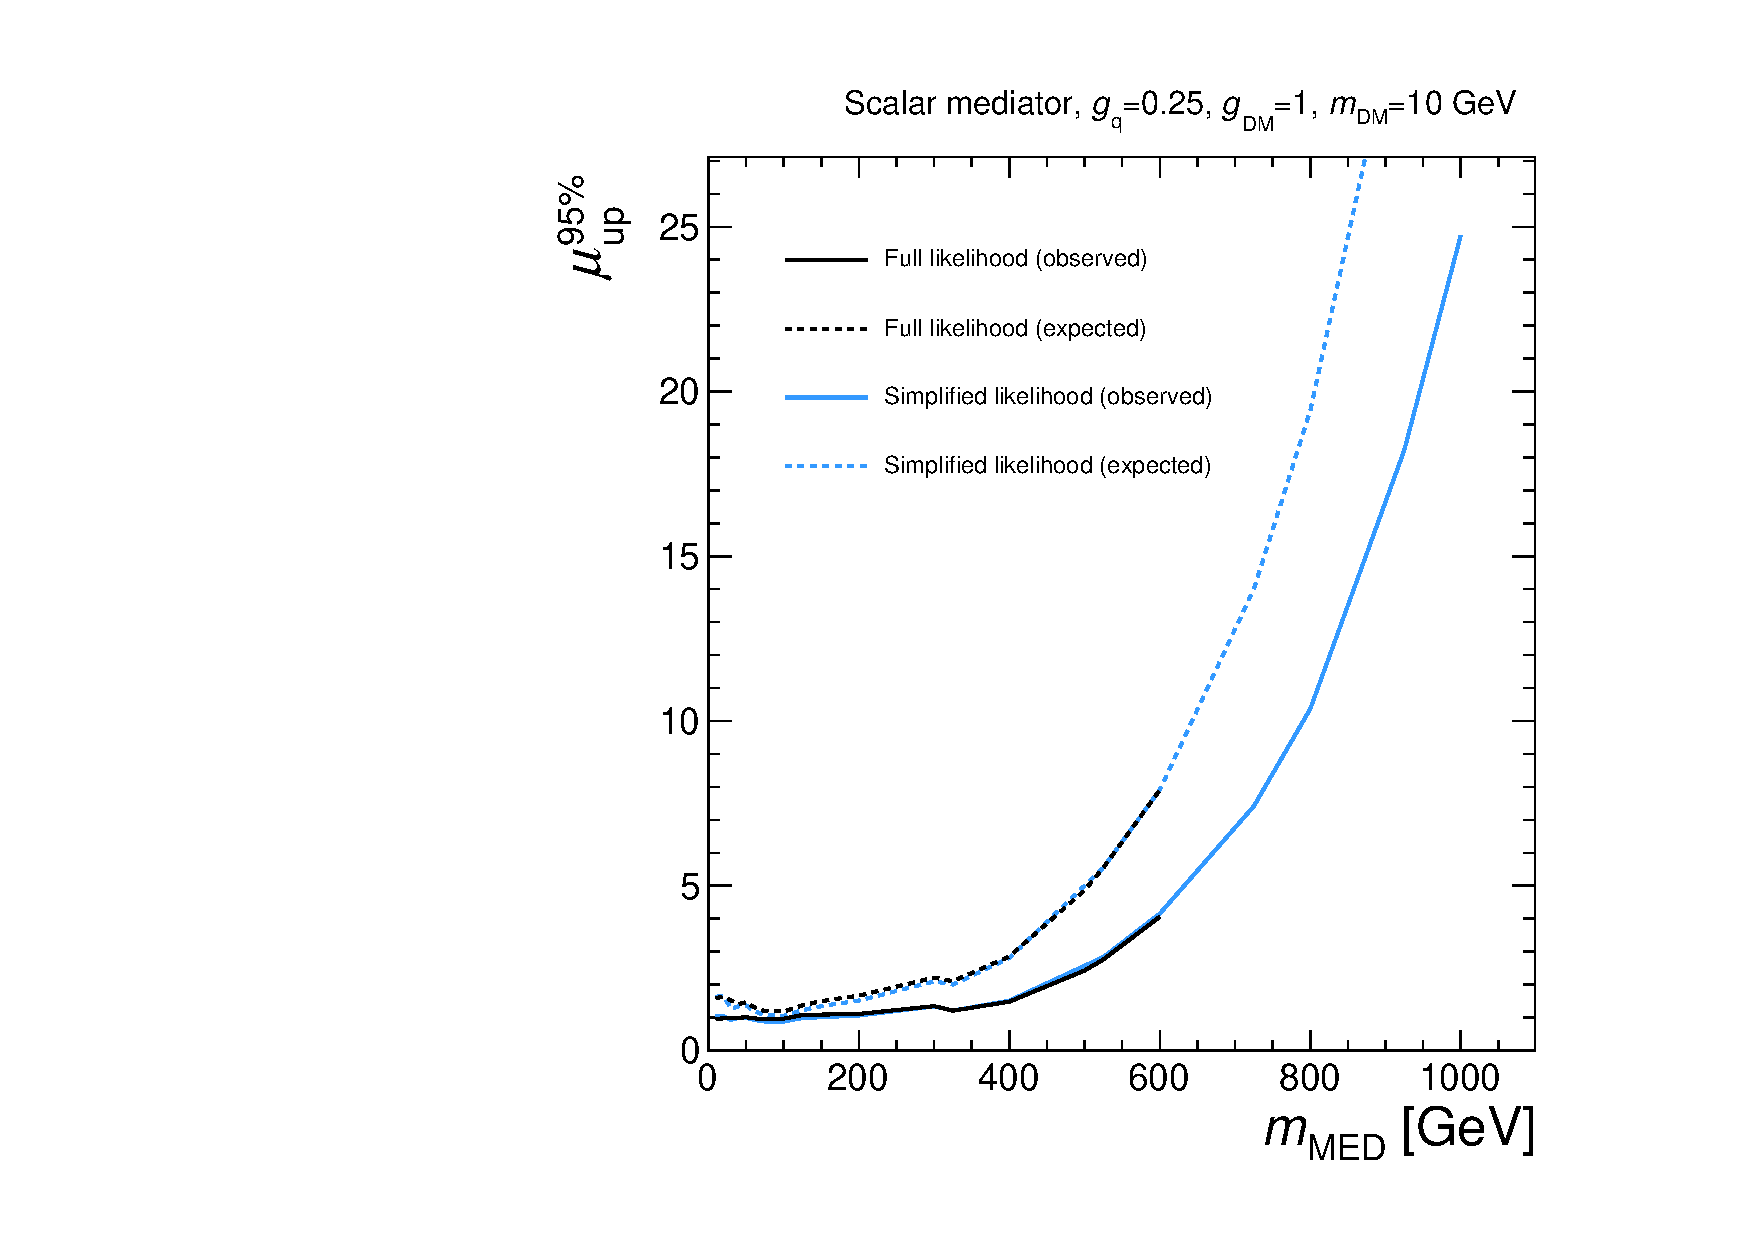
\includegraphics[width=1.2\cmsFigWidth]{figures/compare_mj_limits_brazilian_combo_scala.pdf}}
  \subfloat[][]{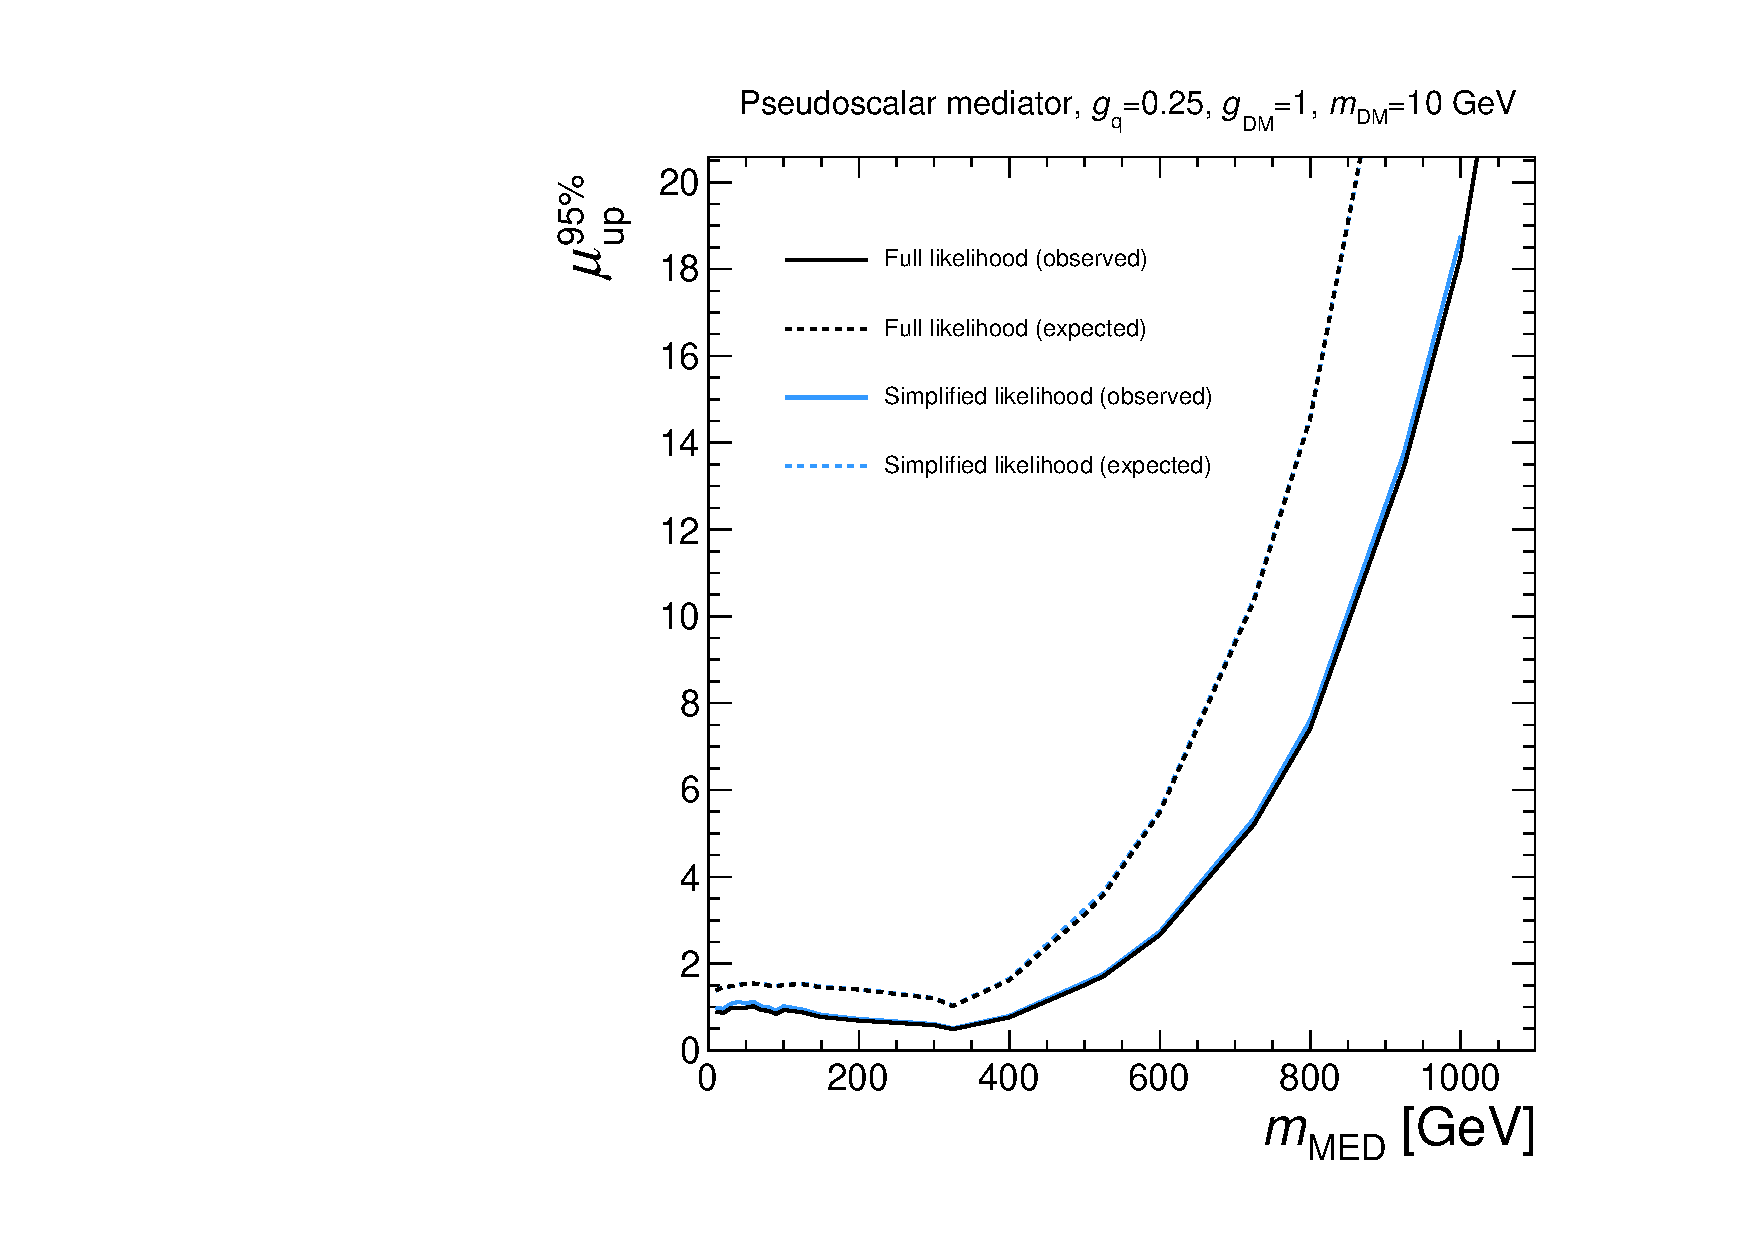
\includegraphics[width=1.2\cmsFigWidth]{figures/compare_mj_limits_brazilian_combo_pseudoscala.pdf}}
   \caption{Expected and observed $\mu_{\mathrm{up}}^{95\%}$ as a function of $m_{\mathrm{MED}}$ for a (a) scalar or (b) pseudoscalar mediator. The results 
   are compared between the limits calculated using the full and the simplified likelihoods.}
   \label{fig:mulims} 
  \end{center}
\end{figure}


Figure~\ref{fig:masslims} shows a comparison of the limits set in the $m_{\mathrm{MED}}$--$m_{\mathrm{DM}}$ plane for a vector or axial vector mediatior with 
fixed coupling parameters using the full and simplified likelihoods. The ratios of the observed values of 
$\mu_up^{95\%}$ between the two likelihood constructions is shown in the color scale. The contours bound the regions for which the observed and expected values of 
$\mu_up^{95\%}$ are less than 1 in the two cases.


\begin{figure}[hbt!]
  \begin{center} 
  \subfloat[][]{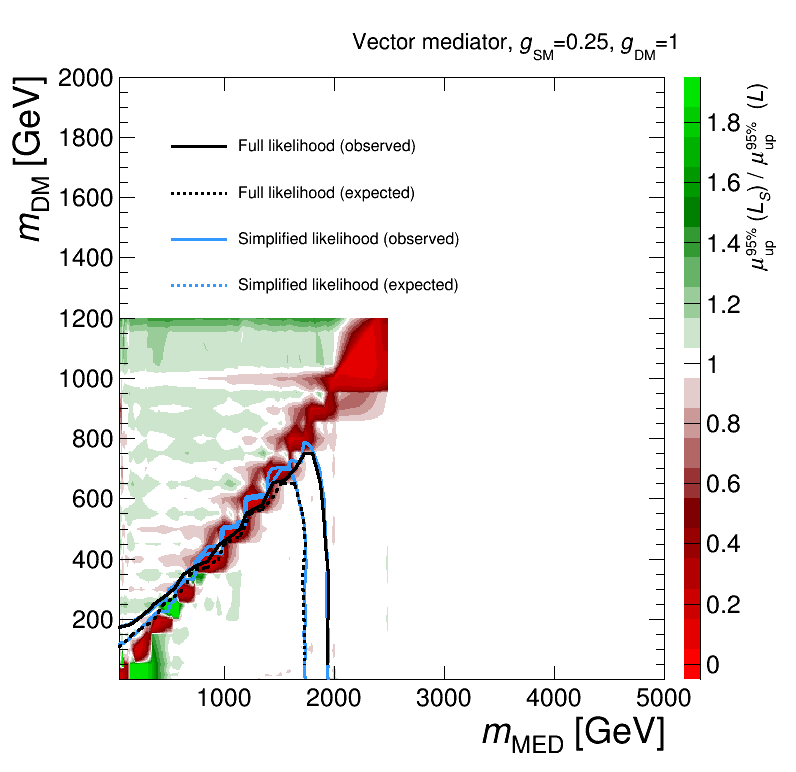
\includegraphics[width=1.2\cmsFigWidth]{figures/compare_mj_limits_scan_combined_vec.png}}
  \subfloat[][]{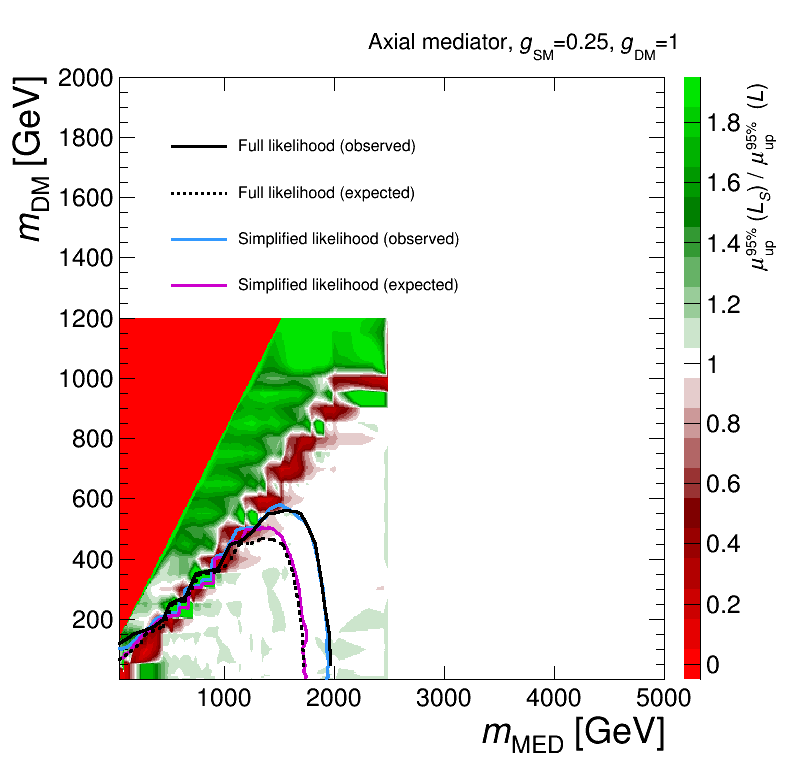
\includegraphics[width=1.2\cmsFigWidth]{figures/compare_mj_limits_scan_combined_axial.png}}
   \caption{Expected and observed exclusion contours defined as the region where $\mu_{\mathrm{up}}^{95\%}\lt1$ in the $m_{\mathrm{MED}}$--$m_{\mathrm{DM}}$ 
   for a (a) vector or (b) axial vector mediator. The results 
   are compared between the limits calculated using the full and the simplified likelihoods. The color scale shows the ratio of $\mu_{\mathrm{up}}^{95\%}$ calculated 
   using the simplified likelihood to the value using the full likelihood.}
   \label{fig:masslims} 
  \end{center}
\end{figure}

